\section{Diagramma Use-Case \& Use-Cases}

    \subsection{Diagramma Use-Case}

        \begin{figure} [H]
            \centering
            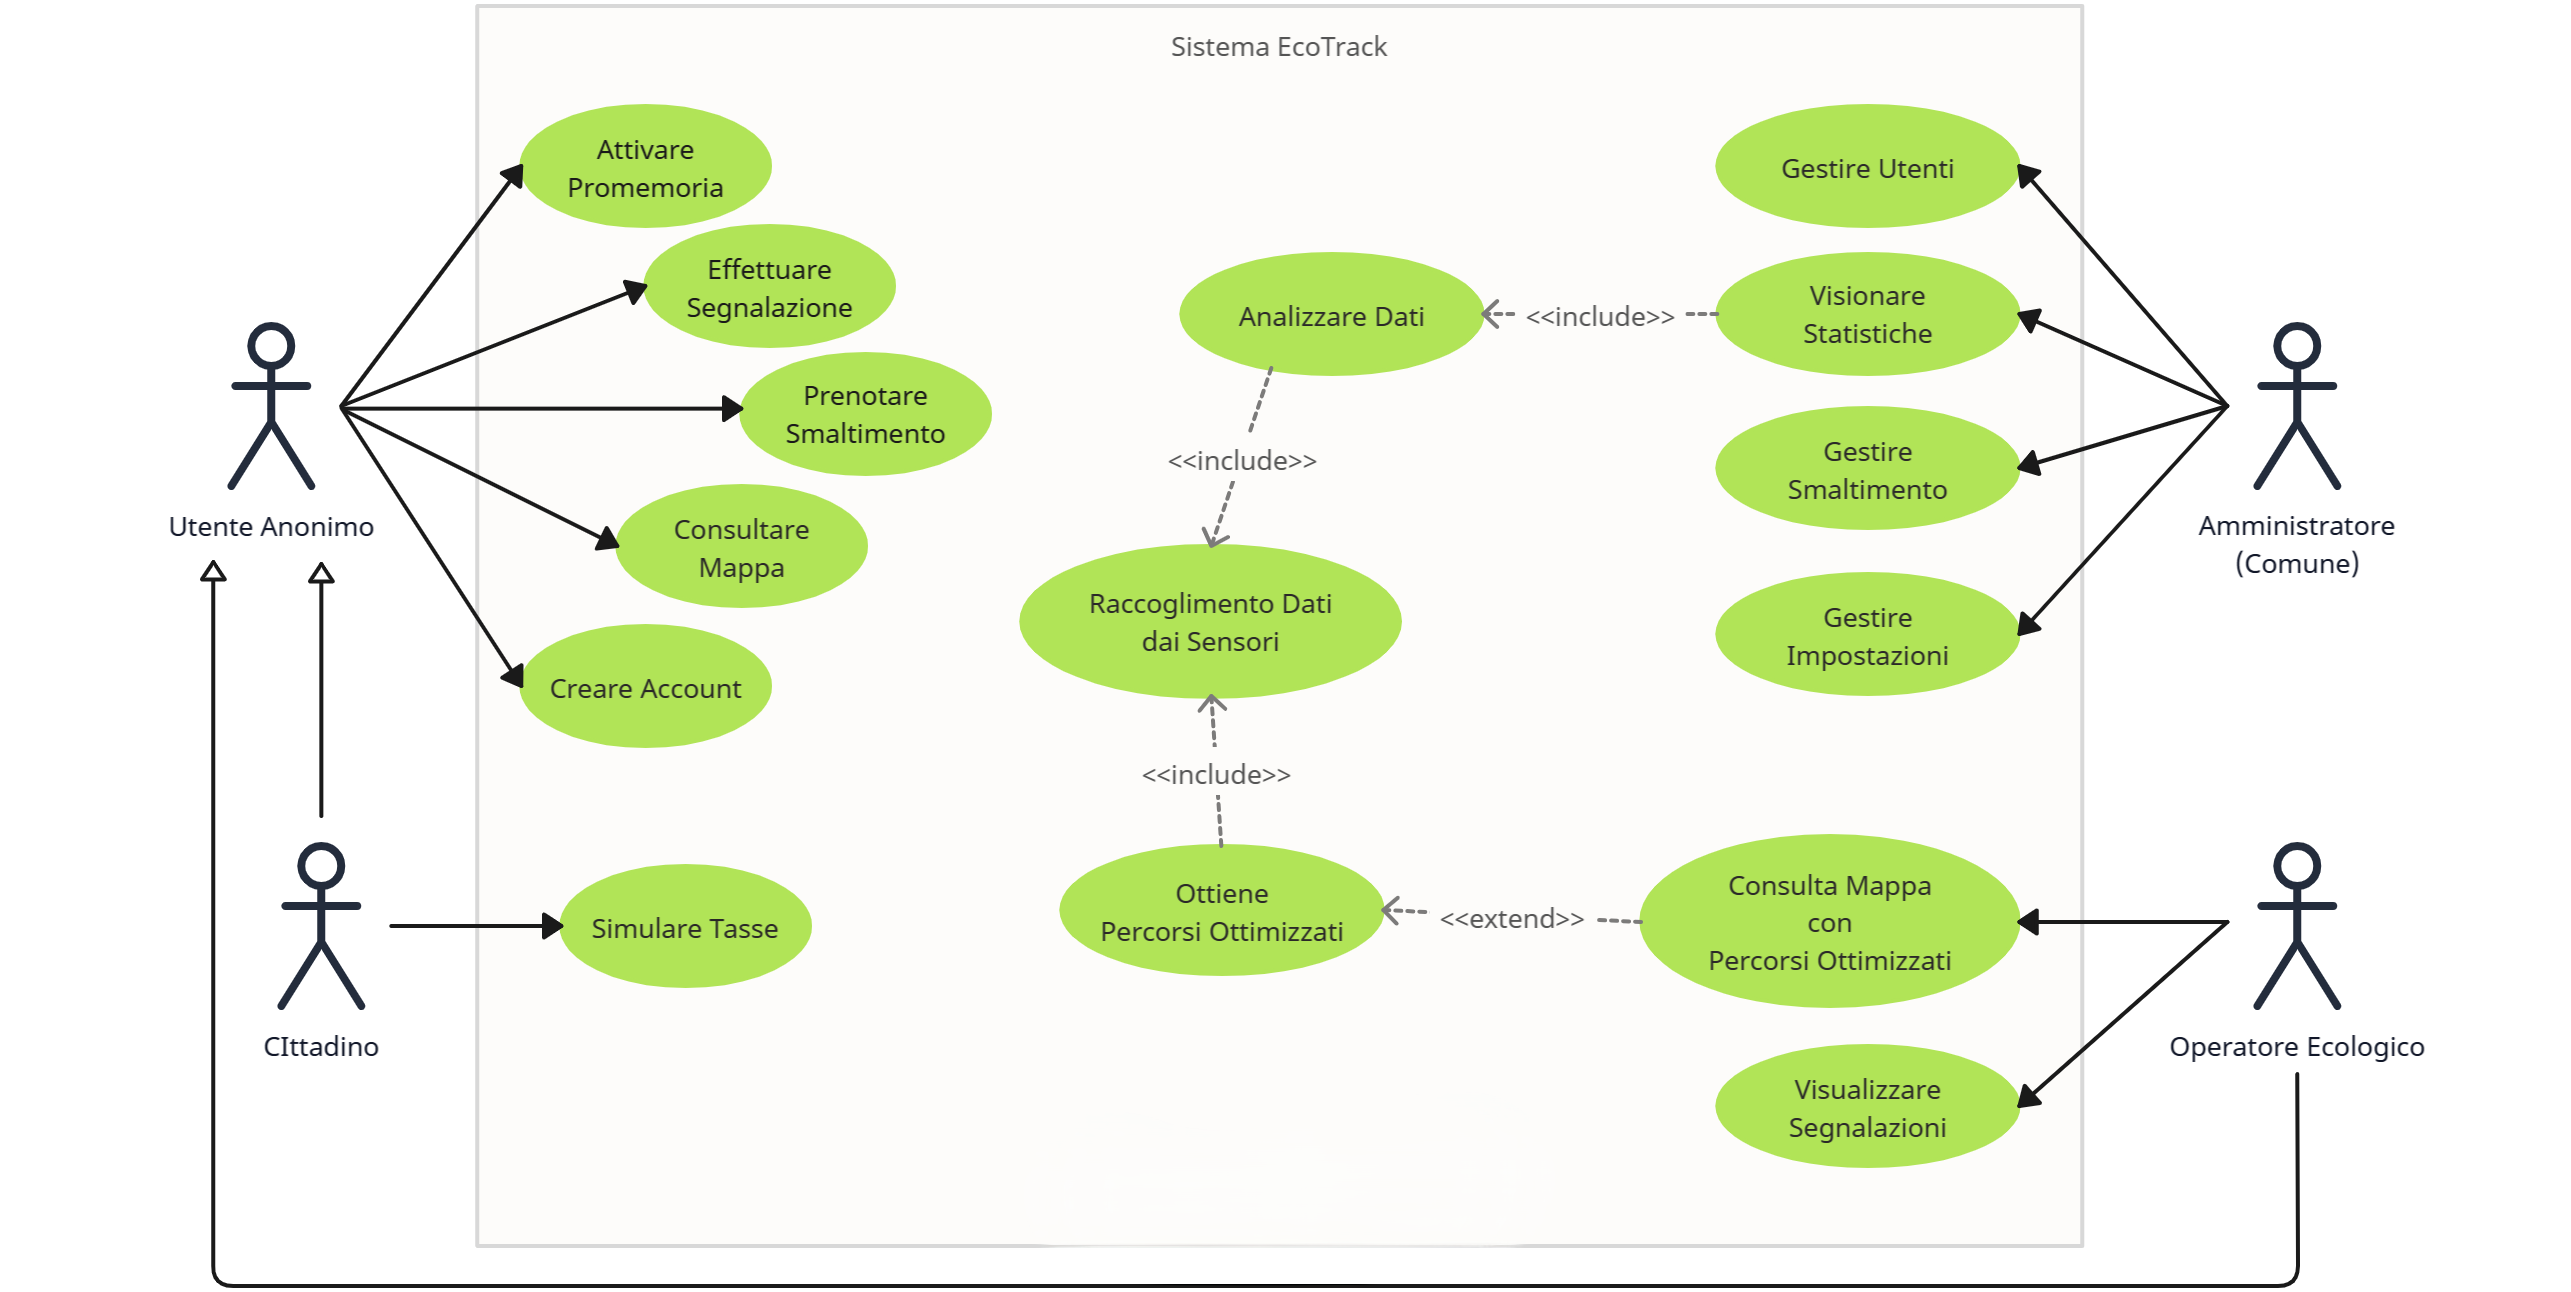
\includegraphics[width=1\linewidth]{D1-G1//Img/Use-Case Diagram - D1.png}
            \caption{Diagramma Use-Case}
            \label{fig:enter-label}
        \end{figure}

    \subsection{Use-Cases}

        \begin{table}[h]
            \centering
            \renewcommand{\arraystretch}{1.3} % Aumenta lo spazio tra le righe
            \begin{tabular}{|p{4cm}|p{10cm}|}
                \hline
                \textbf{Nome Use-Case}& \textbf{Consultare Mappa}\\
                \hline
                \textbf{Id} & UC1   \\
                \hline
                \textbf{Descrizione}& L'utente può accedere ad una mappa interattiva che gli permetta di vedere in tempo reale il livello
                                    di riempimento dei cassonetti, cestini e punti di raccolta temporanei nella sua zona.\\
                \hline
                \textbf{Attori Primari}& Utente Anonimo, Cittadino\\
                \hline
                \textbf{Attori Secondari}& Nessuno\\
                \hline
                \textbf{Pre-Condizioni}& Nessuna\\
                \hline
                \textbf{Flusso Principale}& 
                \begin{enumerate}
                    \item L'attore primario seleziona "\textbf{Mappa Interattiva}"
                    \item Il sistema mostra la mappa
                    \item L'attore primario può consultare la mappa
                \end{enumerate}
                \\
                \hline
                \textbf{Post-Condizioni}& L'attore primario ha consultato la mappa\\
                \hline
                \textbf{Flusso Alternativo}& Errore di caricamento della mappa\\
                \hline
            \end{tabular}
            \caption{Use-Case Table per Consulta Mappa}
            \label{tab:use_case}
        \end{table}

        \begin{table}[h]
            \centering
            \renewcommand{\arraystretch}{1.3} % Aumenta lo spazio tra le righe
            \begin{tabular}{|p{4cm}|p{10cm}|}
                \hline
                \textbf{Nome Use-Case}& \textbf{Consulta Mappa con Percorsi Ottimizzati}\\
                \hline
                \textbf{Id} & UC2   \\
                \hline
                \textbf{Descrizione}& L'operatore ecologico può accedere ad una mappa interattiva che gli permetta di vedere in tempo reale il livello
                                    di riempimento dei cassonetti nella sua zona e che gli consenta di ottenere e visualizzare dei percorsi ottimizzati\\
                \hline
                \textbf{Attori Primari}& Operatore Ecologico\\
                \hline
                \textbf{Attori Secondari}& Nessuno\\
                \hline
                \textbf{Pre-Condizioni}& Avere eseguito l'accesso in qualità di operatore ecologico.\\
                \hline
                \textbf{\hyperref[fig:BPMN] {Flusso Principale}}& 
                \begin{enumerate}
                    \item L'attore primario seleziona "\textbf{Mappa Interattiva}"
                    \item Il sistema mostra la mappa
                    \item L'attore primario può consultare la mappa e richiedere percorsi ottimizzati
                    \item  \textbf{Se} i cassonetti pieni sono maggiori o uguali ad un threshold
                \begin{enumerate}
                    \item Il sistema restituisce i percorsi ottimizzati, mostrandoli all'interno della mappa
                \end{enumerate}
                \item  \textbf{Altrimenti}
                \begin{enumerate}
                    \item Il sistema non restituisce alcun percorso
                \end{enumerate}
                \end{enumerate}
                \\
                \hline
                \textbf{Post-Condizioni} & L'attore primario ha consultato la mappa ed (eventualmente) ottenuto i percorsi ottimizzati richiesti \\
                \hline
                \textbf{Flusso Alternativo}& Errore di caricamento della mappa \\
                \hline
                \textbf{Punti di estensione}& Al passo 3: Ottiene Percorsi Ottimizzati\\
                \hline
            \end{tabular}
            \caption{Use-Case Table per Consulta Mappa con Percorsi Ottimizzati}
            \label{tab:use_case}
        \end{table}

        \begin{table}[h]
            \centering
            \renewcommand{\arraystretch}{1.3} % Aumenta lo spazio tra le righe
            \begin{tabular}{|p{4cm}|p{10cm}|}
                \hline
                \textbf{Nome Use-Case}& \textbf{Ottiene Percorsi Ottimizzati}\\
                \hline
                \textbf{Id} & UC3 \\
                \hline
                \textbf{Descrizione}& Vengono calcolati percorsi ottimizzati, basandosi sulla raccolta dati dei sensori\\
                \hline
                \textbf{Attori Primari}& Operatore ecologico\\
                \hline
                \textbf{Attori Secondari}& Nessuno\\
                \hline
                \textbf{Pre-Condizioni}& L'operatore ecologico deve aver richiesto la visione di percorsi ottimizzati mediante la mappa, come mezionato nello UC2\\
                \hline
                \textbf{Flusso Principale}& 
                \begin{enumerate}
                    \item Include(Raccoglie i Dati Sensori)
                    \item Il sistema elabora i dati ottenuti dai sensori e propone un percorso ottimizzato
                \end{enumerate}
                \\
                \hline
                \textbf{Post-Condizioni}& L'attore primario ottiene il percorso ottimizzato\\
                \hline
                \textbf{Flusso Alternativo}& Errore di caricamento del percorso\\
                \hline
            \end{tabular}
            \caption{Use-Case Table per Ottiene Percorsi Ottimizzati}
            \label{tab:use_case}
        \end{table}

        \begin{table}[h]
            \centering
            \renewcommand{\arraystretch}{1.3} % Aumenta lo spazio tra le righe
            \begin{tabular}{|p{4cm}|p{10cm}|}
                \hline
                \textbf{Nome Use-Case}& \textbf{Effettuare Segnalazione}\\
                \hline
                \textbf{Id} & UC4 \\
                \hline
                \textbf{Descrizione}& L'utente compila un form, allegando foto, per segnalare la presenza di rifiuti abbandonati nelle aree della città\\
                \hline
                \textbf{Attori Primari}& Utente Anonimo, Cittadino\\
                \hline
                \textbf{Attori Secondari}& Nessuno\\
                \hline
                \textbf{Pre-Condizioni}& Nessuna\\
                \hline
                \textbf{Flusso Principale}&
                \begin{enumerate}
                    \item L'attore primario seleziona "\textbf{Segnalazioni}"
                    \item Il sistema mostra un form da compilare
                    \item L'attore primario invia la segnalazione con eventuale foto allegata
                    \item Il sistema salva la segnalazione nel database interno
                \end{enumerate}
                \\
                \hline
                \textbf{Post-Condizioni} & La segnalazione contenuta nel database è pronta per essere visionata dall'operatore ecologico o dall'amministrazione\\
                \hline
                \textbf{Flusso Alternativo}& Errore di invio segnalazione\\
                \hline
            \end{tabular}
            \caption{Use-Case Table per Effettua Segnalazione}
            \label{tab:use_case}
        \end{table}

        \begin{table}[h]
            \centering
            \renewcommand{\arraystretch}{1.3} % Aumenta lo spazio tra le righe
            \begin{tabular}{|p{4cm}|p{10cm}|}
                \hline
                \textbf{Nome Use-Case}& \textbf{Gestire Smaltimento}\\
                \hline
                \textbf{Id} & UC5\\
                \hline
                \textbf{Descrizione}& L'amministratore può visionare una dashboard con i vari stati di riempimento e le richieste di smaltimento\\
                \hline
                \textbf{Attori Primari}& Amministratore\\
                \hline
                \textbf{Attori Secondari}& Nessuno\\
                \hline
                \textbf{Pre-Condizioni}& Avere effettuato l'accesso in qualità di amministratore\\
                \hline
                \textbf{Flusso Principale}& 
                \begin{enumerate}
                    \item L'attore primario seleziona "\textbf{Gestione Smaltimento}"
                    \item Il sistema mostra una lista degli stati di riempimento dei vari ecocentri e le richieste di smaltimento
                \end{enumerate}
                \\
                \hline
                \textbf{Post-Condizioni} & I vari stati e le richieste sono stati mostrati \\
                \hline
                \textbf{Flusso Alternativo}& Errore di caricamento dei vari stati e richieste \\
                \hline
            \end{tabular}
            \caption{Use-Case Table per Gestisce Smaltimento}
            \label{tab:use_case}
        \end{table}

        \begin{figure}[h]
            \centering
            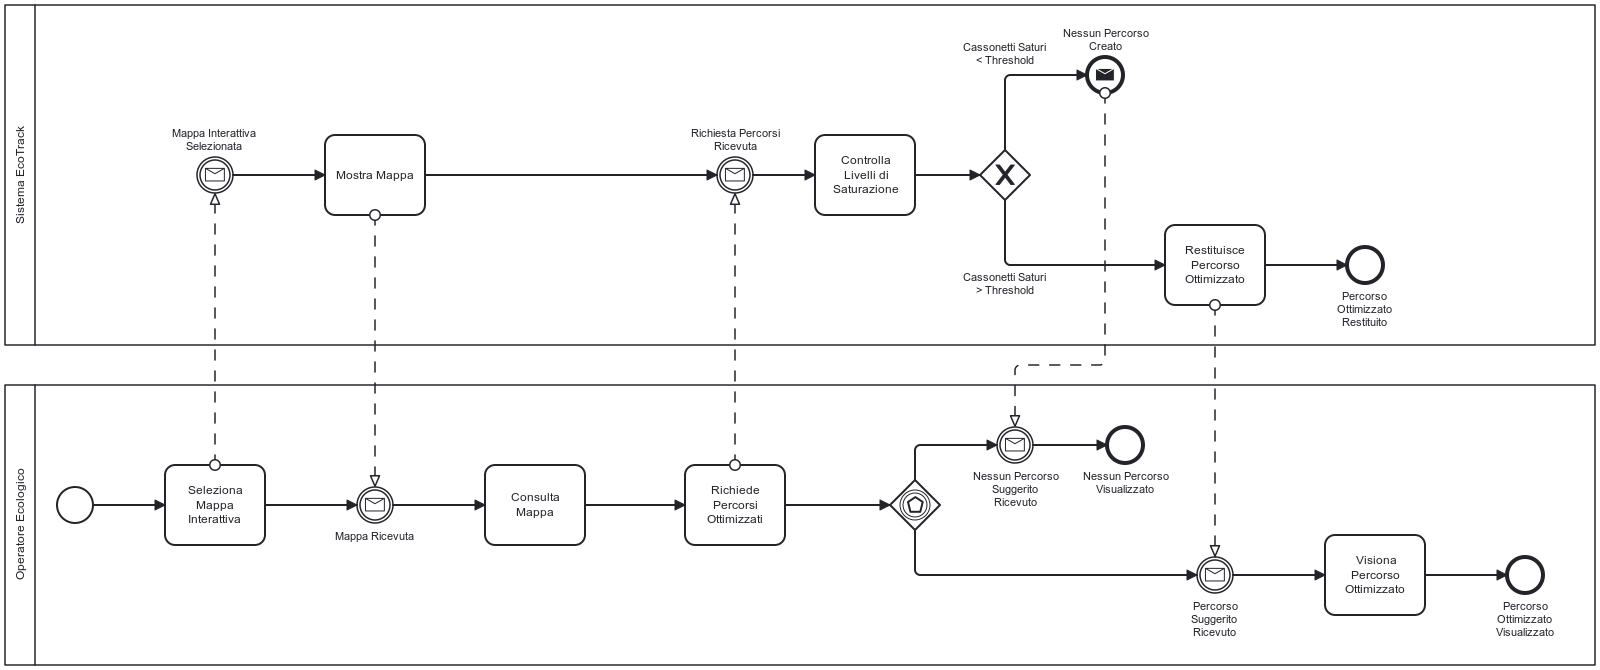
\includegraphics[width=1\linewidth]{D1-G1//Img/Consulta Mappa - BPMN.png}
            \caption{Diagramma BPMN per UC2}
            \label{fig:BPMN}
        \end{figure}